% Options for packages loaded elsewhere
\PassOptionsToPackage{unicode}{hyperref}
\PassOptionsToPackage{hyphens}{url}
\documentclass[
]{article}
\usepackage[a4paper,top=3cm,bottom=3cm,left=4cm,right=3cm]{geometry}
\usepackage{xcolor}
\usepackage{amsmath,amssymb}
\setcounter{secnumdepth}{-\maxdimen} % remove section numbering
\usepackage{iftex}
\ifPDFTeX
  \usepackage[T1]{fontenc}
  \usepackage[utf8]{inputenc}
  \usepackage{textcomp} % provide euro and other symbols
\else % if luatex or xetex
  \usepackage{unicode-math} % this also loads fontspec
  \defaultfontfeatures{Scale=MatchLowercase}
  \defaultfontfeatures[\rmfamily]{Ligatures=TeX,Scale=1}
\fi
\usepackage{lmodern}
\ifPDFTeX\else
  % xetex/luatex font selection
\fi
% Use upquote if available, for straight quotes in verbatim environments
\IfFileExists{upquote.sty}{\usepackage{upquote}}{}
\IfFileExists{microtype.sty}{% use microtype if available
  \usepackage[]{microtype}
  \UseMicrotypeSet[protrusion]{basicmath} % disable protrusion for tt fonts
}{}
\makeatletter
\@ifundefined{KOMAClassName}{% if non-KOMA class
  \IfFileExists{parskip.sty}{%
    \usepackage{parskip}
  }{% else
    \setlength{\parindent}{0pt}
    \setlength{\parskip}{6pt plus 2pt minus 1pt}}
}{% if KOMA class
  \KOMAoptions{parskip=half}}
\makeatother
\usepackage{graphicx}
\makeatletter
\newsavebox\pandoc@box
\newcommand*\pandocbounded[1]{% scales image to fit in text height/width
  \sbox\pandoc@box{#1}%
  \Gscale@div\@tempa{\textheight}{\dimexpr\ht\pandoc@box+\dp\pandoc@box\relax}%
  \Gscale@div\@tempb{\linewidth}{\wd\pandoc@box}%
  \ifdim\@tempb\p@<\@tempa\p@\let\@tempa\@tempb\fi% select the smaller of both
  \ifdim\@tempa\p@<\p@\scalebox{\@tempa}{\usebox\pandoc@box}%
  \else\usebox{\pandoc@box}%
  \fi%
}
% Set default figure placement to htbp
\def\fps@figure{htbp}
\makeatother
\setlength{\emergencystretch}{3em} % prevent overfull lines
\providecommand{\tightlist}{%
  \setlength{\itemsep}{0pt}\setlength{\parskip}{0pt}}
\usepackage{bookmark}
\IfFileExists{xurl.sty}{\usepackage{xurl}}{} % add URL line breaks if available
\urlstyle{same}
\hypersetup{
  hidelinks,
  pdfcreator={LaTeX via pandoc}}

\author{}
\date{}

\begin{document}

\textbf{Tugas 1}

STSI4310 -- Metodologi Penelitian

\textbf{Gate Klasifikasi Terkalibrasi sebagai Kendali Tulis Memori Agen
Pi: Akurasi, Kalibrasi, dan Biaya}

\textless Nama Mahasiswa\textgreater{} - \textless NIM\textgreater{}

Program Studi Sistem Informasi

Fakultas Sains dan Teknologi

Universitas Terbuka

2026

\textbf{DAFTAR ISI}

\textbf{DAFTAR ISI i}

\textbf{BAB I PENDAHULUAN 1}

\begin{quote}
1.1 Latar Belakang Masalah 1

1.2 Rumusan Masalah 4

1.3 Tujuan Penelitian 5

1.4 Manfaat Penelitian 6
\end{quote}

\textbf{BAB II KAJIAN PUSTAKA DAN LANDASAN TEORI 7}

\begin{quote}
2.1 Kajian Pustaka dan Landasan Teori 7

2.2 Pertanyaan Penelitian dan Hipotesis 7
\end{quote}

\textbf{BAB III METODE PENELITIAN 8}

\begin{quote}
3.1 Metode Penelitian 8

3.2 Teknik Pengumpulan Data dan Instrumen Penelitian 8
\end{quote}

\textbf{BAB IV ANALISIS DATA DAN KESIMPULAN SEMENTARA 9}

\begin{quote}
4.1 Teknik Analisis Data Penelitian 9

4.2 Kesimpulan Sementara dan Batasan Penelitian 9
\end{quote}

\textbf{DAFTAR PUSTAKA 10}

\textbf{BAB I PENDAHULUAN}

\textbf{1.1 Latar Belakang Masalah}

Coding agent seperti Pi bekerja per sesi. Ketika sesi ditutup, konteks
yang sudah terbangun di dalamnya ikut hilang: preferensi pengguna,
konvensi repositori, keputusan arsitektur yang pernah diambil, kegagalan
tool yang pernah terjadi, dan pekerjaan yang belum selesai. Kehilangan
ini bukan sekadar ketidaknyamanan, karena setiap sesi baru memaksa
pengguna mengulang penjelasan yang sama dan agen mengulang kesalahan
yang sama. Ekosistem Pi menjawab masalah tersebut dengan extension
memori yang menyimpan pengetahuan lintas sesi.\emph{pi-memory}, yang
menyimpan memori dalam berkas markdown, log harian, dan scratchpad
dengan pencarian semantik opsional, serta \emph{pi-hermes-memory}, hasil
port dari agen Hermes, yang menyimpan memori berkategori dengan
pencarian SQLite FTS5, pemindaian rahasia, dan skills prosedural
(Dokumentasi paket \emph{pi-memory} dan \emph{pi-hermes-memory}, 2026).
Keduanya adalah contoh perangkat lunak yang perilakunya berubah karena
data yang ia simpan sendiri, sehingga mutu keputusan menyimpan menjadi
bagian dari mutu sistem.

Persoalan yang diangkat penelitian ini bukan pada kemampuan menyimpan,
melainkan pada cara keputusan menulis diambil. Kedua extension tersebut
menjalankan dua peran berbeda dengan satu model generatif yang sama:
model itu menilai apakah sebuah informasi layak diingat, lalu model yang
sama merumuskan teks entri memori yang disimpan. \emph{pi-hermes-memory}
menjalankan review latar setiap 10 turn atau 15 tool call, mendeteksi
koreksi pengguna, lalu menulis entri melalui side-channel di dalam
proses. \emph{pi-memory} mengekspor ringkasan pada peristiwa compaction
dan menyediakan tool tulis yang dipanggil model. Penyatuan dua peran
pada satu model generatif ini membawa dua konsekuensi yang dapat diukur.

Konsekuensi pertama adalah biaya. Setiap penilaian kelayakan adalah
panggilan model generatif penuh, dan panggilan itu terjadi berulang
sepanjang sesi tanpa memandang apakah ada informasi yang benar-benar
layak disimpan. Penilaian juga menempati jendela konteks, karena riwayat
yang sedang dinilai harus disertakan. Sebagai pembanding, model
keputusan terstruktur seperti Jev dari TypeSafe AI menerima state dan
peta pertanyaan, lalu mengembalikan tiga jenis nilai terketik, yaitu
\emph{choice} (memilih satu label), \emph{score} (skala terurut), dan
\emph{noul} (probabilitas untuk jawaban ya atau tidak), dalam satu round
trip berlatensi puluhan sampai ratusan milidetik, pada kisaran harga
masukan 0,42 dolar per juta token atau sekitar 0,001 dolar per keputusan
dan konteks maksimum 64 ribu token (TypeSafe AI, 2026). Selisih orde
biaya dan latensi inilah yang membuat pemisahan peran layak diuji.

Konsekuensi kedua adalah ketidakreproduksian dan ketidakpastian yang
tidak terukur. Model generatif yang diminta menilai kelayakan memberi
jawaban berbeda untuk masukan yang sama, dan angka keyakinan yang
dilaporkannya ditulis sebagai bagian dari teks, bukan dihasilkan sebagai
nilai probabilitas. Akibatnya dua hal yang seharusnya dapat dipisahkan
menjadi tercampur: perubahan mutu memori tidak dapat dibedakan dari
variasi sampling model, dan ambang keputusan tidak dapat dipilih secara
bertanggung jawab karena angka yang menjadi dasarnya tidak bermakna
secara statistik. Dokumentasi Jev sendiri mengingatkan bahwa nilai
keyakinan menunjukkan seberapa terkonsentrasi jawaban, bukan jaminan
kebenaran, dan menyarankan kalibrasi ambang terhadap data berlabel milik
pemakai (TypeSafe AI, 2026). Peringatan itu menjadi salah satu
pertanyaan penelitian ini, bukan asumsinya.

Di sisi industri, pemisahan peran tersebut sudah ditunjukkan sebagai
arah yang masuk akal. Command Code memakai model neuro-simbolik taste-1
yang bukan model generatif: ia menerima sinyal terstruktur berupa
accept, reject, dan diff koreksi, lalu memutuskan apakah sinyal itu
preferensi yang nyata, kategori mana yang sesuai, dan seberapa tinggi
keyakinannya. Lapisan simboliknya memelihara daftar kategori tetap dan
menandai konflik alih-alih menimpa preferensi lama, sementara model
generatif hanya dipakai untuk membaca sinyal dan menuliskan hasilnya
sebagai markdown (Command Code, 2026). Klaim di balik rancangan itu
jelas: keputusan yang deterministik dengan keyakinan terkalibrasi lebih
dapat dipercaya daripada angka keyakinan yang dikarang model generatif.

Di sisi akademik, kendali pada sisi tulis atau write-side control sudah
tumbuh menjadi subbidang tersendiri, bukan lagi pelengkap retrieval.
SAGE merumuskan evolusi memori sebagai masalah deteksi kebaruan dan
memakai gate tertutup tanpa panggilan model generatif untuk memisahkan
fakta baru, fakta redundan, dan kasus ambigu yang baru dilempar ke model
generatif (Wang dkk., 2026). ConsistencyGate merumuskan admission
sebagai masalah kebenaran, bukan kegunaan, dan menambahkan benchmark uji
kontaminasi memori (Zhang \& Li, 2026). A-MEM memformalkan admission
sebagai gate terpisah dengan skor kegunaan hasil pembelajaran (Xu dkk.,
2025). Perkembangan itu menunjukkan satu hal yang sama: keputusan
menulis adalah sumber biaya sekaligus sumber kegagalan jangka panjang,
karena fakta yang salah dan lolos akan terus dipakai sebagai premis pada
langkah berikutnya.

Namun tiga celah masih terbuka. Pertama, celah konteks. Benchmark memori
jangka panjang yang mapan, seperti LoCoMo (Maharana dkk., 2024),
LongMemEval (Wu dkk., 2025), dan MemBench (MemBench, 2025), bertumpu
pada percakapan chat atau interaksi pengguna dengan asisten. Memori
kerja coding agent punya distribusi yang berbeda: isinya keputusan
teknis, konvensi repositori, kegagalan tool, dan koreksi atas keluaran
model. LongMemEval-V2 mulai bergerak ke memori pengalaman agen, tetapi
pada agen web dan dengan fokus pengetahuan lingkungan, bukan sesi
pemrograman (Wu dkk., 2026). Kedua, celah evaluasi. Evaluasi penolakan
pada saat penulisan atau write-time rejection sebagai keputusan
tersendiri, dengan ground truth berlabel dan laporan kesepakatan antar
annotator, masih jarang. Penelitian write-time trust gating yang
menyusun 113 kasus berlabel dan 12 mode kegagalan, dan melaporkan
Cohen\textquotesingle s kappa 0,475, bahkan menyatakan celah ini sebagai
kontribusi utamanya (TIMPS Research, 2026). Ketiga, celah instrumen dan
kalibrasi. Gate yang sudah ada dievaluasi pada akurasi atau penghematan
biaya, tetapi jarang dievaluasi pada kalibrasi, padahal dua gate yang
sama-sama akurat dapat berbeda jauh nilainya ketika keyakinannya dipakai
sebagai ambang: gate dengan keyakinan berlebih akan meloloskan kasus
yang seharusnya dieskalasi. Literatur kalibrasi modern sudah menunjukkan
bahwa jaringan saraf modern cenderung terlalu percaya diri dan bahwa
kalibrasi post-hoc seperti temperature scaling dapat memperbaikinya
tanpa mengubah prediksi (Guo dkk., 2017). Karena itu membandingkan
classifier terlatih dengan model yang memang dilatih untuk terkalibrasi,
tanpa memberi kesempatan kalibrasi post-hoc kepada classifier terlatih,
adalah perbandingan yang tidak adil. Rancangan penelitian ini menjaga
keadilan perbandingan tersebut.

Dengan demikian, pertanyaan yang diajukan penelitian ini bersifat
spesifik. \emph{Jika peran penilaian dipisahkan dari model generatif dan
diserahkan kepada classifier terkalibrasi, apakah akurasi gate tetap
setara dengan LLM judge, apakah nilai keyakinannya cukup terkalibrasi
untuk dipakai sebagai ambang keputusan, dan berapa ongkos pemisahan itu
dalam token, biaya, serta latensi?} Pertanyaan itu berada di ruang
lingkup Sistem Informasi karena menyangkut perancangan dan evaluasi
komponen sistem berbasis kecerdasan artifisial, bukan sekadar pelatihan
model: yang diuji adalah rancangan kendali pada jalur tulis sebuah
perangkat lunak agen, beserta konsekuensinya pada biaya operasional dan
mutu data yang disimpan sistem.

\textbf{1.2 Rumusan Masalah}

Berdasarkan latar belakang di atas, akar masalah penelitian ini dapat
dipetakan pada diagram tulang ikan berikut.

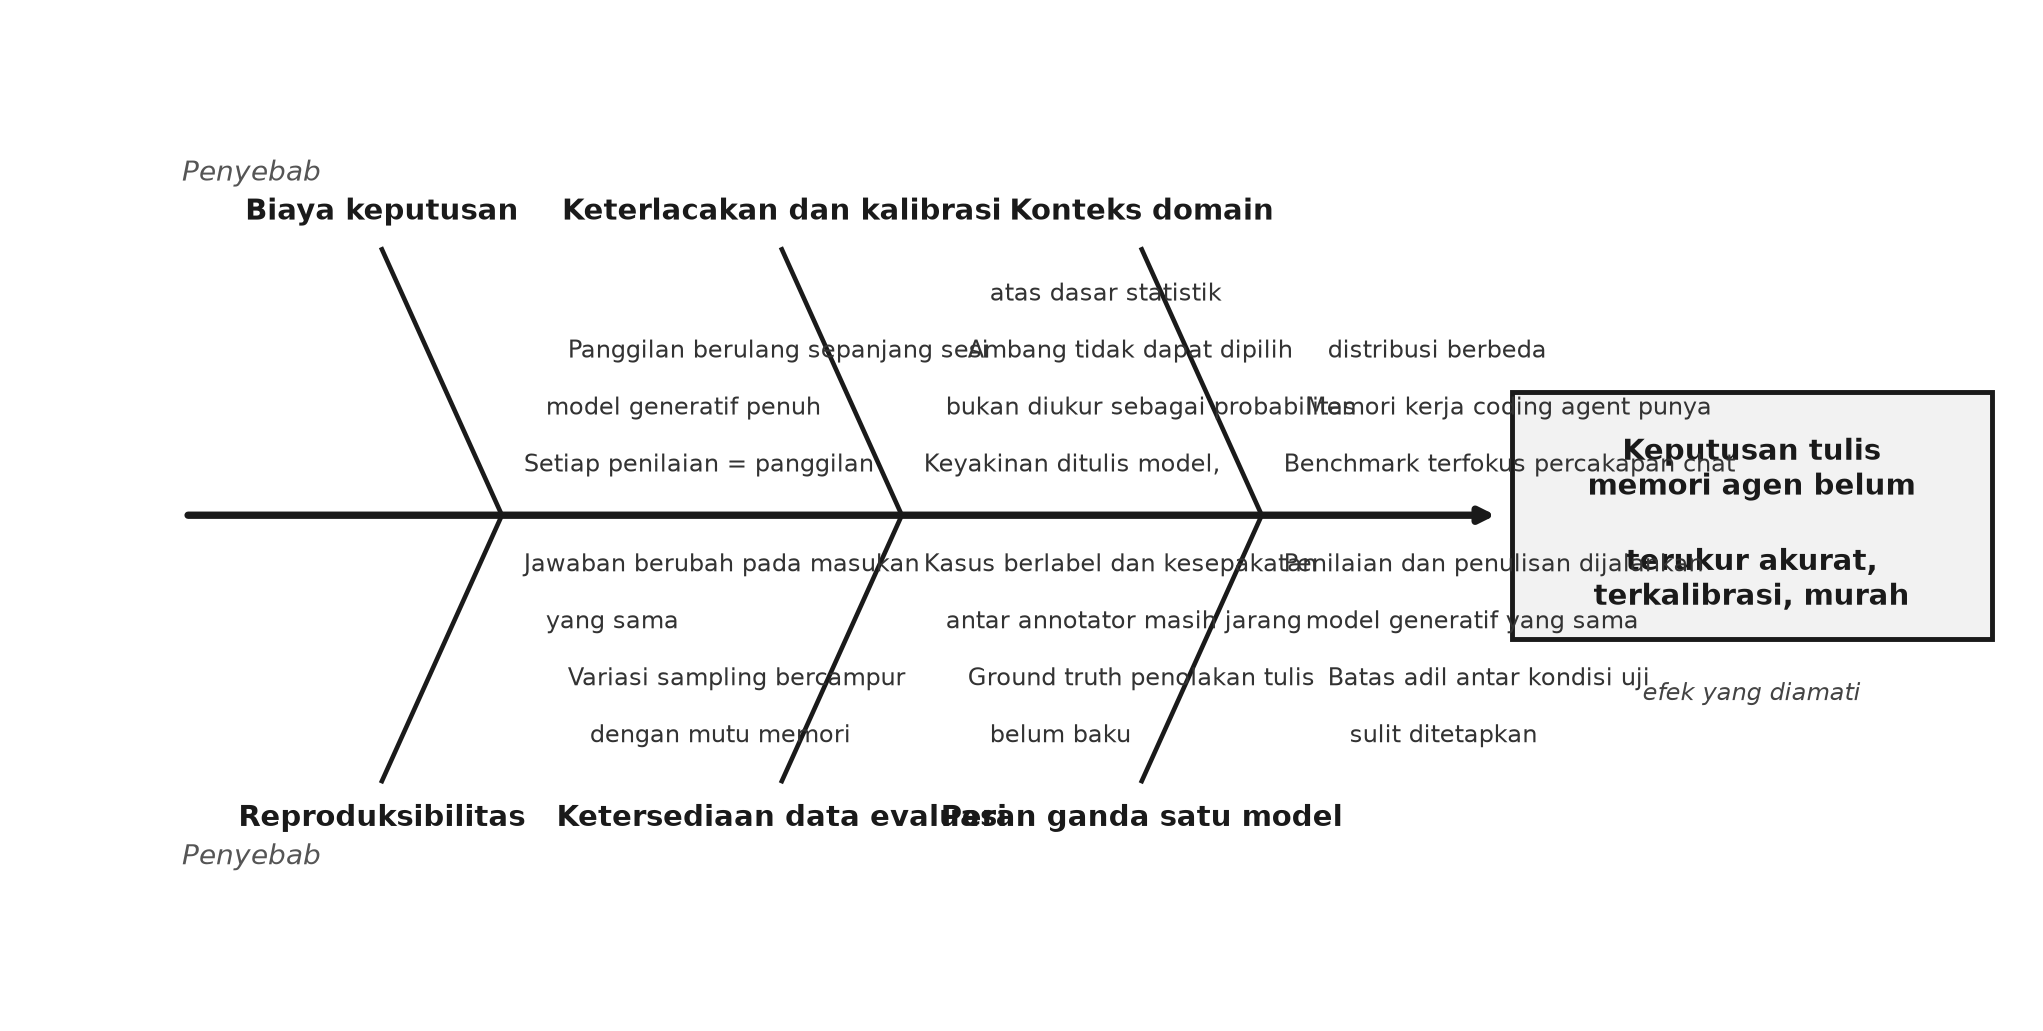
\includegraphics[width=5.70866in,height=2.88088in]{./media/image1.png}

\emph{Gambar 1.1 Diagram tulang ikan akar masalah keputusan tulis memori
agen}

Rumusan masalah penelitian ini disusun dalam bentuk pertanyaan
penelitian sebagai berikut.

\begin{quote}
1. Sejauh mana akurasi gate keputusan tulis yang dipisahkan dari model
generatif berbeda dari LLM judge yang merangkap peran penilaian dan
penulisan, pada tugas kelayakan simpan memori sesi coding agent?

2. Apakah classifier terlatih dan model keputusan terkalibrasi berbeda
secara bermakna pada akurasi gate, dan apakah pemberian kalibrasi
post-hoc kepada classifier terlatih menutup perbedaan tersebut?

3. Apakah nilai keyakinan masing-masing gate terkalibrasi pada tugas
ini, dan apakah ambang yang dipilih berdasarkan hasil kalibrasi
mengalahkan ambang tetap?

4. Berapa token, biaya, dan latensi per 1.000 operasi tulis pada setiap
kondisi, dan bagaimana bentuk kurva trade-off antara akurasi dan biaya
pemisahan peran tersebut?

5. Apakah mekanisme band ketidakpastian, yaitu terima otomatis, tolak
otomatis, dan eskalasi ke LLM hanya pada rentang tengah, memangkas
panggilan model generatif tanpa penurunan bermakna pada mutu memori dan
akurasi probe QA pada sesi lanjutan?
\end{quote}

\textbf{1.3 Tujuan Penelitian}

Sejalan dengan rumusan masalah di atas, penelitian ini bertujuan untuk:

\begin{quote}
1. Memisahkan peran penilaian kelayakan dari peran penulisan entri pada
jalur tulis memori ekosistem Pi dan mengimplementasikannya sebagai
extension dengan satu pintu kendali.

2. Menyusun dataset berlabel untuk tugas kelayakan simpan memori sesi
coding agent, lengkap dengan pedoman anotasi dan laporan kesepakatan
antar annotator.

3. Membandingkan lima pendekatan keputusan tulis, yaitu heuristik tanpa
model, deteksi kebaruan berbasis embedding, classifier terlatih, model
keputusan terkalibrasi, dan LLM judge, pada empat ukuran: akurasi gate,
kalibrasi, biaya, dan latensi.

4. Menguji apakah kalibrasi post-hoc menyetarakan classifier terlatih
dengan model yang dilatih untuk terkalibrasi, sehingga dapat dipisahkan
mana yang berpengaruh terhadap hasil, akurasi atau kalibrasi.

5. Menguji secara empiris apakah band ketidakpastian berbasis keyakinan
terkalibrasi layak dipakai sebagai strategi eskalasi selektif.
\end{quote}

\textbf{1.4 Manfaat Penelitian}

\textbf{Manfaat teoritis.} Penelitian ini menguji klaim kalibrasi sebuah
model keputusan terstruktur di luar domain aslinya, yaitu routing tugas,
pada domain penilaian kelayakan memori. Hasilnya memperkaya pembahasan
write-side control pada domain memori kerja coding agent yang belum
banyak diteliti.

\textbf{Manfaat praktis.} Penelitian ini memberi ekosistem Pi mekanisme
memori yang lebih murah dan lebih deterministik pada keputusan tulisnya,
tanpa mengubah cara entri memori ditulis. Pemakai extension memori juga
memperoleh gambaran biaya, token, dan latensi per 1.000 operasi tulis,
yang dapat dipakai untuk memilih rancangan kendali sesuai anggaran
pemakaian.

\textbf{Manfaat metodologis.} Penelitian ini menyediakan protokol
evaluasi admission sisi tulis untuk domain memori coding agent, yang
memuat pengukuran kalibrasi dan kesepakatan antar annotator, tidak hanya
akurasi dan penghematan biaya.

\textbf{BAB II KAJIAN PUSTAKA DAN LANDASAN TEORI}

\textbf{2.1 Kajian Pustaka dan Landasan Teori}

\emph{{[}KOSONGKAN. Bagian ini diisi pada Tugas 2.{]}}

\textbf{2.2 Pertanyaan Penelitian dan Hipotesis}

\emph{{[}KOSONGKAN. Bagian ini diisi pada Tugas 2.{]}}

\textbf{BAB III METODE PENELITIAN}

\textbf{3.1 Metode Penelitian}

\emph{{[}KOSONGKAN. Bagian ini diisi pada Tugas 3.{]}}

\textbf{3.2 Teknik Pengumpulan Data dan Instrumen Penelitian}

\emph{{[}KOSONGKAN. Bagian ini diisi pada Tugas 3.{]}}

\textbf{BAB IV ANALISIS DATA DAN KESIMPULAN SEMENTARA}

\textbf{4.1 Teknik Analisis Data Penelitian}

\emph{{[}KOSONGKAN. Bagian ini diisi pada Tugas 4.{]}}

\textbf{4.2 Kesimpulan Sementara dan Batasan Penelitian}

\emph{{[}KOSONGKAN. Bagian ini diisi pada Tugas 4.{]}}

\textbf{DAFTAR PUSTAKA}

Chhikara, P., Khant, D., Aryan, S., Singh, T., \& Yadav, D. (2025).
Mem0: Building production-ready AI agents with scalable long-term memory
(arXiv:2504.19413). arXiv. https://arxiv.org/abs/2504.19413

Chow, C. K. (1970). On optimum recognition error and reject tradeoff.
IEEE Transactions on Information Theory, 16(1), 41--46.

Command Code. (2026). Taste dan taste-1: Dokumentasi resmi Command Code.

Dokumentasi paket pi-memory dan pi-hermes-memory. (2026). Arsitektur
jalur tulis memori extension coding agent.

Earendil Works. (2026). Pi coding agent: Dokumentasi extension (paket
@earendil-works/pi-coding-agent versi 0.87.1).

Guo, C., Pleiss, G., Sun, Y., \& Weinberger, K. Q. (2017). On
calibration of modern neural networks. Dalam Proceedings of the 34th
International Conference on Machine Learning (hlm. 1321--1330). PMLR.

Maharana, A., Lee, D.-H., Tulyakov, S., Bansal, M., Barbieri, F., \&
Fang, Y. (2024). Evaluating very long-term conversational memory of LLM
agents (arXiv:2402.17753). arXiv. https://arxiv.org/abs/2402.17753

MemBench: Towards more comprehensive evaluation on the memory of
LLM-based agents. (2025). Dalam Findings of the Association for
Computational Linguistics: ACL 2025.

Evaluating memory in LLM agents via incremental multi-turn interactions
(MemoryAgentBench). (2026). Dalam International Conference on Learning
Representations (ICLR).

Packer, C., Wooders, S., Lin, K., Fang, V., Patil, S. G., Stoica, I., \&
Gonzalez, J. E. (2023). MemGPT: Towards LLMs as operating systems
(arXiv:2310.08560). arXiv. https://arxiv.org/abs/2310.08560

TIMPS Research. (2026). Write-time trust gating for LLM memory systems.

TypeSafe AI. (2026). System One Models dan Jev: Dokumentasi resmi,
termasuk batasan kalibrasi dan anjuran pin versi model.

Wang, S., Brahma, D., \& Henao, R. (2026). SAGE: A novelty gate for
efficient memory evolution in agentic LLMs (arXiv:2605.30711). arXiv.
https://arxiv.org/abs/2605.30711

Wu, D., Ji, Z., Kawatkar, A., Kwan, B., Gu, J.-C., Peng, N., \& Chang,
K.-W. (2026). LongMemEval-V2: Evaluating long-term agent memory toward
experienced colleagues (arXiv:2605.12493). arXiv.
https://arxiv.org/abs/2605.12493

Wu, D., Wang, H., Yu, W., Zhang, Y., Chang, K.-W., \& Yu, D. (2025).
LongMemEval: Benchmarking chat assistants on long-term interactive
memory. Dalam International Conference on Learning Representations
(ICLR).

Xu, W., Liang, Z., Mei, K., Gao, H., Tan, J., \& Zhang, Y. (2025).
A-MEM: Agentic memory for LLM agents (arXiv:2502.12110). arXiv.
https://arxiv.org/abs/2502.12110

Zhang, Y., \& Li, S. (2026). ConsistencyGate: Preventing memory
contamination in LLM agents via self-consistency admission control
(arXiv:2607.22962). arXiv. https://arxiv.org/abs/2607.22962

\end{document}
